\chapter{Contribution}
\label{ch:Contribution}
In this chapter, we discuss the features and changes introduced in this thesis as well as other implementation options and why we chose our approaches over the others. In the following sections, in lack of a better term, observable is used as a term to denote an actual RxJS observable but also as a placeholder for any reactive entity from RxJS or BaconJS depending on the context.

\section{Advancing the User Interface}
The User Interface (UI) is an important part of every application. A good UI helps the user focus on the task at hand by displaying the necessary information required for that task. For a website this task may simply be to gather information about the subject of the website itself. An IDE usually provides a number of tools to reduce the manual work of the user by automating parts of the development process. There are many factors that need to be taken into account when developing a new UI or changing an existing one. A UI should be designed to match an applications specific use-cases while also keeping some familiar elements to guide the user. The main reason for including familiar elements is simplicity for the user: If the UI elements look familiar and match a user's expectations, it is much easier for the user to handle the UI as there are not as many features a user needs to learn how to use. In fact, it is also important to consider some of the characteristics of human cognition which we will not discuss in detail due to the limited scope of this thesis.
  
\textbf{Reducing the cognitive load on the user}\\
The main goal of the changes to the UI we implemented in this thesis is to reduce the cognitive load on the user. The user should not need to actively look for information in the UI; Instead the UI should present its functions and information in an easily accessible manner. This way, the user spends more attention on their actual task and less attention on finding the information. The first change we introduced to reduce the cognitive load on the user is to move some input elements to a menu that is displayed at the top of the CRI's UI. Nearly every desktop application and many websites (e.g. http://reactivex.io/rxjs/, Windows File Explorer, Eclipse, Microsoft Paint, Adobe PDF Reader and many more) use a menu at the top of the UI. This adds structure and also removes many buttons from the normal working space which can then be used to display more relevant information. The user knows that the buttons are in the menu and opens it on demand. Except for the space required by the menu itself, the buttons hidden in the menu bar do not require space or attention by the user at other times. We examined our own usage frequency, i.e. how often we use a certain input element, and estimated the tasks that include the input element to determine which elements should be part of the main UI and which should be hidden in a menu (or closeable panel for inputs other than buttons). We found that we rarely use the \emph{Reset}, \emph{Download} and \emph{Pause/Resume} buttons. The latter was used most among them and since the CRI does not actually have many buttons yet, we decided to place it directly in the menu bar instead of moving it into the submenu where we placed the other rarely used buttons. The \emph{Pause/Resume} button is also the only one of those buttons used in a normal workflow, i.e. in the special case of working with rapidly updated observables (see section \ref{sec:RapidlyUpdatedObservables}) it is used regularly to counter performance issues or focus on a specific part of the execution. The other buttons of the UI are each part of a specific feature of the CRI and cannot be moved away from other elements which belong to that feature. These features from left top to bottom right are the \emph{instrumented files list}, \emph{history queries} and the navigation through their results, \emph{reactive breakpoints}, \emph{search}, \emph{history navigation} and the \emph{dependency graph}. The dependency graph and history navigation are closely tied together and represent the main part of the CRI. They are the working area where the focus of the UI should be. The other features are complementary to them and support the user in examining their content. Although \emph{history queries} and \emph{reactive breakpoints} are not needed to effectively use the CRI, they can help the user in almost any task. \emph{Reactive breakpoints} may even be mandatory to discover issues with an application that otherwise could not be detected without a much greater effort - similar to normal Breakpoints in traditional IDEs. \emph{Reactive breakpoints} are currently exclusive to the CRI, while the dependency graph with its history is just an alternative to the marble diagrams used in RxFiddle to abstractly represent observables and dependencies. In conclusion, \emph{history queries} and \emph{reactive breakpoints} should be a permanent part of the UI. We therefore decided to keep them where they were positioned in the CRI2 - above the history navigation.
The search feature is not as important in most tasks. Searching and highlighting a specific node, its dependencies or dependents, is only useful for applications with large dependency graphs; In small graphs it is easier to find nodes manually. Therefore, the search feature could be moved to a closable panel that opens on demand similar to the search implementation in most IDEs where a user presses CTRL F or clicks the button in the menu to open the search bar. The reason we did not move the feature to a closable panel yet is simply that the area of the UI where the history query and \emph{reactive breakpoints} are placed provides enough space, with standard screen resolutions for desktop computers, to keep the search there as well. With the current UI, this space is otherwise left empty. However, as soon as these parts of the UI change or another feature is introduced, the search should be moved to a closable panel. The remaining feature is the \emph{instrumented files list}. It is used as a scoping feature to select which files should be instrumented. For small to medium-sized applications the list of files will normally include all relevant JS files and will not be changed at all. It is, therefore, reasonable to move it from the main UI to free the space that could then be used to increase the size of the dependency graph's canvas. After examining the outcome of this change we found, however, that in case the user switches to another application that requires other files to be instrumented or forgot to include a JS file in the list, it is really difficult to detect the reason why the dependency graph is not showing the expected result. If the Instrument Files list is moved from the main UI, the user may lose track of the fact that not all JS files are automatically instrumented or, if they decided to instrument only a subset of JS files as a filtering measure, that this filter is still in place. It is also easier for new users to comprehend the need to select files for instrumentation if the list is part of the main UI. This could be mitigated by adding a dialog informing the user at the first start of the CRI, but for this reason, in addition to the reasons mentioned above, we decided the benefits outweigh the downside of a small part of the UI being occupied by a rarely changed input. Therefore, we kept the \emph{instrumented files list} at the top of the UI and also added a red border around the text input in case the list is empty to help make new users aware of the missing input.

To further decrease the cognitive load when working with the CRI, we removed any text from nodes and their tooltips that does not carry any value. The less text is displayed in the UI, the less a user needs to read to find the information they require. This is most significant for the \emph{Method} field in the tooltips since most observables do not correspond to a method and the field, therefore, is empty for most nodes. The \emph{Value} field is usually set, but in case no value is available, there is no need to keep the label for the field. No information is lost if the field label for \emph{Value} is simply omitted in that case.
It is, however, important to display values that explicitly denote an \emph{empty} value like \emph{undefined}, \emph{null}, or ,in case of a value that carries positive numbers if it is set, -1. The \emph{Name} field is also not set for every node. Figure \ref{fig:Nodes} shows an example of nodes from the CRI2 with all fields as well as nodes from the current version.
\begin{figure}[!h]
	\centering
	\subfloat[CRI version 2.0]{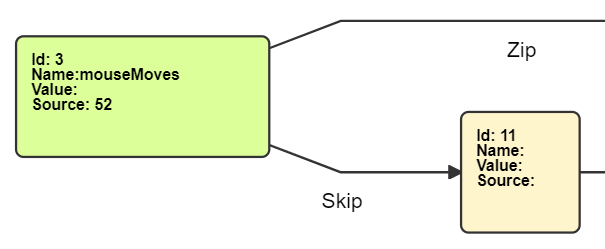
\includegraphics[width=0.4\textwidth]{gfx/NodesCRI2.png}\label{fig:NodesCRI2}}
	\hfill
	\subfloat[CRI version 3.0]{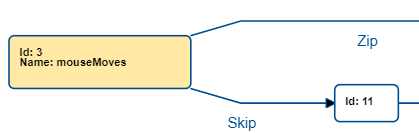
\includegraphics[width=0.4\textwidth]{gfx/NodesCRI3.png}\label{fig:NodesCRI3}}
	\caption{A sample of nodes before and after the changes introduced by this thesis.}
	\label{fig:Nodes}
\end{figure}
Another important aspect to consider is if to display a field directly on the node or rather in the tooltip. The same principle that applies to general elements of the UI applies here as well. Only values for which it is necessary to always have them present, without the need to open every tooltip, should be displayed as part of the nodes. We evaluated for each field where they should be located regarding this criteria. The \emph{Name} is important to identify relevant nodes, including those depending or dependent on such a \emph{named} node. The \emph{Id} is required to add \emph{reactive breakpoints} and to identify nodes without a name from one step to another in case the nodes are repositioned due to a new edge being added. The \emph{Value} is usually the property that lets developers see if the JS code of the application works as intended. This can be achieved for example by checking if an observable fulfills the expectation of having a specific value at a specific point in the execution. The developer is also able to observe a value passing along the chain of dependencies. For these reasons, the fields \emph{Name}, \emph{Id} and \emph{Value}, as long as they have a value, should always be displayed as part of the node.
The \emph{Type} should be hidden in the tooltip, because often what type of observable the library uses internally does not matter to the user. For example in most scenarios for RxJS, there is no difference between a \emph{FromEventObservable} and a basic \emph{Observable}. The information should, however, be still present in the tooltip and not omitted completely because some types of observables do behave differently than others such as an RxJS's \emph{subject} in contrast to its \emph{observables}. The source code position labeled \emph{Source} is also just used in few special tasks. One example is the user wanting to find the source code corresponding to a node in the graph to modify that code or inspect it further. The \emph{Source} should, therefore, be displayed in the tooltip rather than the nodes themselves. The field \emph{Number of Updates} is introduced by this thesis as a way to detect bottlenecks in the performance of the inspected application and to help identify nodes that cause the generation of a huge amount of steps in the CRI through excessive value updates. It is based on the Time Profiling feature of the Reactive Inspector \cite{ReactiveInspector}, but for now, only provides the total number of updates on a node instead of detailed timing and value evaluation information. It is only useful for the purposes mentioned above and, therefore, should not be displayed on the nodes themselves.

An important cognitive task that a user has to do often while using the CRI is to track changes between steps in the dependency graph's history. To track these changes is necessary to understand how the graph is constructed or to track value updates traveling along a chain of dependent observables. It is, however, not always trivial since the rendering engine \emph{D3.js} \cite{D3JS} used by the CRI sometimes moves nodes and edges around to better fit the available space. To help the user with this task, the previous version of the CRI already highlighted the nodes that were changed for each step in which a node was changed. We extended this feature to also highlight edges that were updated or added to further decrease the manual searching process. Another feature we added to the UI is a button that hides the tool section of the UI - everything except the menu, history navigation and dependency graph - to allow the user to reduce distractions and free up additional space if they want to focus on the manual examination of the graph and its history. The button is located at the top right corner and has a small arrow icon instead of a text label to reduce its required space in the UI. The option to hide the tool section is especially useful when working with a small screen or a large dependency graph. Another button we added to the UI, as part of the menu, was a button to reload the inspected page and, therefore, the dependency graph as well. We discovered that reloading was already part of the usual workflow by pressing CTRL F5 and decided to add a button that allows users to achieve this without being aware of the shortcut. An example workflow in which a reload can be used is to create a \emph{dependencyCreated} or \emph{nodeCreated} breakpoint for a node which is already displayed in the dependency graph, and then reloading the application to actually hit the breakpoint.
As figure \ref{fig:Nodes} shows, we also changed the colors used in the CRI UI. The node which was changed in the currently viewed step was highlighted by using a red border in the previous version of the CRI. The color red is a signal color normally used to show that immediate attention is required or to show that an error has occurred. In traffic signs and lights the color red is used to signal cars to stop or to be aware of dangers. Therefore, we decided to remove it from the normal workflow of the CRI. Highlighting the current node is important for the user to immediately identify the change between steps, but it does not require the user's full attention the whole time. It also neither represents an error, therefore the increased cognitive load on the user is unnecessary. The combination of red and green (\emph{named} nodes are colored green) is also problematic for some users with a fairly common vision deficiency, although as the green is a very bright shaded they should still be able to distinguishable the border on a highlighted \emph{named} node from the node itself. Because of these reasons we decided to use blue with light orange as the highlighting that has less contrast between the two shades but still enough to not void the highlighting. To this purpose, we chose a shade of blue and selected the colors for nodes, edges and highlighting from suggestions provided by a color scheme designer \cite{Paletton}. We chose to keep the text color black because it is the most used color for text in general and is easy to read on most colored backgrounds. The nodes that do not correspond to a named variable were left without a background to further reduce the cognitive load. The brain is trained to ignore empty spaces, therefore, making the text and named nodes appear more important.

Another change we introduced to the UI of the CRI was the automatic reloading of the dependency graph if the \emph{instrumented files list} is changed. This does not reduce the cognitive load on the user but removes the redundant click on the reload button. It is not very useful to change the list of instrumented files without restarting the inspected application and the recording. If the reloading is not triggered automatically, the user will even be confused that their changes to the instrumented files list do not take effect immediately.
	
\section{Connecting abstract graph with JavaScript code}
Nodes in the dependency graph that correspond to observables that are directly assigned to variables provide developers with some form of context. A \emph{named} node can be used as an anchor to identify the node itself as well as other nodes up and down the chain of dependencies. It helps the user to separate parts of the dependency graph that are relevant to the piece of code they want to examine and parts that are currently not relevant. Without any orientation, it is very hard to interpret a shown dependency graph. The user can still try to identify nodes by their values or the values of their neighbors, but these values may be missing at certain stages of the application. This all boils down to the issue of connecting the abstract representation of the applications observables provided by the dependency graph with the actual JS source code responsible for the creation of those observables. If an error is detected by examining nodes in the dependency graph, the user still has to track down which lines of code are responsible for the issue in order to change them. As mentioned above, \emph{named} nodes solve this issue in a way, but not all observables created during runtime are assigned to variables. In fact, it is not at all desirable, although this is possible to achieve by editing the source code. To assign the result of each function in a chain of functions to a variable negates most of the benefits of using chained functions in the first place. If the variables are not used by multiple lines of code and are just introduced to support the debugging tool, most of all the disadvantages of \emph{do-debugging} apply here as well. We, therefore, evaluated several possibilities to provide nodes that do not have a corresponding variable in the source code with additional details that help provide some context to the user. A very basic form of context was already present in the previous versions of the CRI in form of the source code position information. This information was, however, not very accurate in case of chained functions because only the line-based start of the source code position information provided by Jalangi was used. In case of chained functions, the source code position actually spans a block that may consist of multiple lines of source code and is character-based. In addition, the information provided by the Jalangi Demo analysis does not contain the name of the JS file to which the position belongs. Another downside of this approach is that to look up the source code in another tool apart from the CRI and switching back to the CRI to check the position of the next node is very cumbersome to execute for more than a few nodes. The developer should be able to easily switch between source code inspection and examining the dependency graph because not all issues can be found in either of them when used alone. For example, if there is an issue in an anonymous function, a user cannot find this issue directly in the dependency graph. They may only see the result in node values that do not match the values that they expect with the original intention of the code in mind. The main difficulty to achieve the connection between the two views on the application by showing actual source code instead of just the position information is that the JS code which is used during runtime is instrumented with Jalangi to enable a detailed analysis. Jalangi instrumented code, however, is very hard to read as is shown in listing \ref{lst:Instrumented}.

\begin{lstlisting}[language=JavaScript, caption={Example of RxJS code.},label={lst:Instrumented}]
$sonWallet = J$.W(593, '$sonWallet', J$.F(585, J$.I(typeof $ === 'undefined' ? $ = J$.R(569, '$', undefined, true, true) : $ = J$.R(569, '$', $, true, true)), false)(J$.T(577, '#wallet-son', 21, false)), J$.I(typeof $sonWallet === 'undefined' ? undefined : $sonWallet), true, true);
$fatherWallet = J$.W(625, '$fatherWallet', J$.F(617, J$.I(typeof $ === 'undefined' ? $ = J$.R(601, '$', undefined, true, true) : $ = J$.R(601, '$', $, true, true)), false)(J$.T(609, '#wallet-father', 21, false)), J$.I(typeof $fatherWallet === 'undefined' ? undefined : $fatherWallet), true, true);
\end{lstlisting}

For example, "J\$.W" signals the analysis engine that a write operation is executed when the function is called. This makes it unfeasible to directly show the instrumented code to the user. In addition to being very hard to read, the instrumentation of the source code is an implementation detail of the CRI and should not be exposed. Additionally, the code position retrieved from the Jalangi analysis corresponds to the position in the original source code without instrumentation. Note that the JS code that is used during runtime is also dynamically loaded and, therefore, cannot be navigated to out of the box with Chrome DevTools navigation API. Although this is mitigated by adding "//\# sourceURL=" with a custom URL to the bottom of a script. Since showing the Jalangi instrumented source code is not useful for a normal user, we decided to tie the custom source URL to a new option called \emph{CRI Developer Mode} which is located in the options page of the CRI. The different approaches discussed in the following section are designed to enable a user to use both the abstract representation and the source code in tandem.
	%TODO -- continue
\subsection{Evaluated possibilities of displaying source code}
\textbf{Using the \emph{chrome.debugger} API}\\
One possible option is to use the \emph{chrome.debugger} API to open and navigate to the corresponding position of a node. To navigate to a line number in a file if the actual file URL, which can differ for dynamically loaded scripts due to many factors, is known is easily possible. For the reasons explained above, however, navigating to the \emph{instrumented} code is not desirable. A non-instrumented version of the source code seems to exist in Chrome's \emph{Source} windows as a dynamic script, but it is not actually used at runtime. This approach provides a user with syntax highlighting through Chrome and other features like search with regular expressions. They are also able to inspect the whole code of the application, if required, not just the piece of code corresponding to a single node. The downside of this approach is that the user needs to leave the UI of the CRI to access the source information. For a single node, this is not an issue, but it is really cumbersome to inspect the source information of multiple nodes, even if the navigation to the position is automated. In addition, it is not possible to highlight the code block that corresponds to the inspected node, which would be especially useful for observables corresponding to the middle of a block of chained functions. The start and end of the block would have to be manually searched for by the user. Another downside that most likely confuses the user, is that some features of Chrome's DevTools work as expected, but others do not and there is no way for the CRI to display this disparity. Due to the fact that the code shown to a user is not actually being executed, all features specific to runtime interaction like breakpoints, direct code evaluation or watches will not be usable. A user familiar with Chrome's debugging capabilities will most likely expect them to work properly. A modification of this approach is to display the code in another IDE than Chrome. As some modern IDE's provide a featured to navigate to a function's declaration (in WebStorm called "Go to declaration") which is more scalable than using a \emph{string} based search for enterprise-sized applications. Although this feature is not available in Chrome, having the user install another IDE and use it in parallel with Chrome will increase the dependencies of the CRI and the development effort coupled with that dependency while still suffering from all the downsides of this approach explained above.\\

\textbf{Using an integrated lightweight IDE}\\
Another possibility is to use a file viewer that is opened, for example, as a closable panel to show the full source code. Depending on the implementation this approach provides full customization options of the code presentation to the user. In theory, advanced syntax highlighting could be applied, i.e. syntax highlighting based on the usage and structure of functions like WebStorm uses to detect classes and other patterns. It is also possible to highlight observables in the source code while the user hovers over the nodes in the dependency graph, or even permanently coloring the source code based on the abstract representation. The main problem with this approach is the development effort required to achieve a viable implementation. There is no library available, that we are aware of, which provides the needed functionality and customization options. To develop such a library ourselves requires nearly the same amount of development effort needed to implement a traditional IDE for JS since it basically is a lightweight JS IDE displayed in a panel of the CRI. Another issue with this solution is, in addition to the required development effort, that nodes which are close in the dependency graph because they share a dependency do not necessarily correspond to lines of code that are located in close proximity of each other. The code may even be split over several JS files in extreme cases which requires additional view options by any lightweight IDE apart from just showing one JS file.\\

\textbf{Mirroring interactions to a non-instrumented copy of the application}\\
An approach that is possible in theory, but will not withstand a detailed evaluation is to mirror any interaction to the inspected application to a copy of it. The idea is to have one application with instrumented JS files, and one where the JS files are not instrumented. This would enable the CRI to use another approach like using the \emph{chrome.debugger} API to display the actual source code used at runtime while retrieving analysis data from the instrumented mirror application. It enables the user to benefit from every feature of Chrome or another IDE when debugging JS. The problems introduced by copying the entire application and mirroring interactions to it, however, go far beyond the doubled resource consumption. One major issue is the actual recording of user interactions to the original application. There are many tools like Katalon Studio \cite{Katalon} using Selenium \cite{Selenium} that can be used to record and replay interactions to a Web application. These tools are often used to automate the testing of Web applications. Most of these tools are, therefore, designed to ignore certain aspects of interactions like the positioning of elements to make the tests more robust against small changes. Although there are some tools that use pixel positions to record and replay interactions. We could however, find not a single tool that records mouse movements and replays them exactly. It is possible to develop a solution ourselves, but the mentioned tools solve many issues such as always replaying the interactions with the exact same screen resolution. This is especially important if the layout of the applications UI reacts to different screen resolutions. Another issue with replaying interactions to the copied website are security restrictions imposed by Chrome (and other modern browsers) itself. Chrome restricts specific interactions when they are performed by Web applications or Chrome extensions instead of a (human) user. This is to protect users from attackers using custom extensions or Web applications. An example of these restricted interactions is the using of Chrome's context menu or the operating system's clipboard. The reasoning to restrict both are similar and are due to the fact that these features are usable to breach boundaries otherwise monitored by Chrome itself or in case of the clipboard by the operating system. Since these interactions are restricted, it is impossible to replay them on the mirror Web application. This voids all other attempts to replay other types of interaction because the two applications will desynchronize eventually. The danger of the two applications becoming desynchronized is also created by observables or JS code which are time sensitive. For example, an observable or function which is scheduled to be executed or updated every few milliseconds and has any side effect such as increasing a value every time the execution happens, needs to be mirrored to the copy exactly to maintain matching values. This also includes any JS code that is execution-order dependent. The same execution order must be maintained, which is especially hard for asynchronous code even though JS's runtime is event-based \cite{EventBasedJS} and does not actually execute code in parallel. In summary, any code dependent on the order of execution or anything timing related has to be mimicked precisely to keep the mirror in sync with the original application. This cannot be guaranteed for all possible applications in a normal runtime environment. \\
 
\textbf{Source Code Tooltips}\\
The solution we decided to implement is an extension to the already present tooltips for nodes in the dependency graph. The tooltip for a node, if the user hovers over it with the mouse pointer, changes to a short snippet of source code which opens if the user presses the CTRL key. The displayed source code corresponds to the code where the observable represented by the node originates from in addition to a few lines of code before and after the relevant code as orientation. The details of the implementation are explained in the next section. This approach, however, has some limitations. If the node belongs to an observable at the end of a long chain of functions or an anonymous function is used which covers several lines, the code piece may actually be too long to show in a tooltip. If the code is not wrapped properly the code will also be hard to read in a tooltip due to the limited space. In addition, it is also not possible to use any kind of tool such as a search feature inside a tooltip. As the tooltips are relatively short, this issue is not too serious because the code snippet can quickly be read altogether. Another limitation of this approach is that it is not possible to view the full source code. However, since the user cannot change the source code in the CRI either, they have to switch to another tool at some point in the debugging process anyway. For now, the Source Code Tooltips do not provide syntax highlighting and, if added in the future, it is important to note that syntax highlighting of short snippets is not very effective in JavaScript. Since JavaScript is a dynamically typed language, in order to correctly highlight language elements beyond keywords, it is necessary to consider how the elements are used in other areas of the source code. The usefulness of Source Code Tooltips is also greatly decreased if a function reference with an identifier instead of an anonymous function is passed to an \emph{observable operator}. Some other patterns like using callbacks that are not realized as anonymous functions or functions that create other functions also have the same issue. An example of this is shown in listing \ref{lst:NonLambdaCallback}. The source code corresponding to the \emph{named} node "fatherWalletValue" ranges from line 4 to 5. If the function declaration is not directly placed nearby and, therefore, shown in the tooltip as well, it is not possible to view the implementation of "createFunction" in the UI of the CRI.

\begin{lstlisting}[language=JavaScript, caption={Example of using a creation function in RxJS.},label={lst:NonLambdaCallback}]
function createFunction(add) {
return (value) => value + add;
}
let fatherWalletValue = sonWalletValue
.map(createFunction(10));
\end{lstlisting}
The greatest benefit of using Source Code Tooltips is that they compliment the dependency graph very well. A user does not have to leave the CRI to view the corresponding source code and the abstract representation is still the focus of the CRI. The tooltips solve the issue of providing additional details for nodes that do not have a corresponding variable name. In fact, they provide additional information for these nodes as well. Using tooltips also has the advantage that they are easy and fast to open and close again. Therefore, the user is able to inspect several tooltips in short sequence. This helps them to find and remember nodes without a corresponding variable name between multiple uses of the CRI by other means than remembering the Ids. The Ids will also change if the user modifies the source code in a way that adds new nodes to the dependency graph or changes the order of existing ones. Another benefit of using Source Code Tooltips is, that we are able to highlight the exact source code block responsible for a node even within a chain of functions. This is similar to the options provided by using a custom lightweight IDE. In contrast to using another \emph{full-fledged} IDE, however, using tooltips inside the CRI does not introduce new dependencies. Another very important feature of using tooltips is that they do not require additional space in the UI. Using a panel that opens on demand as a pop-up or as part of the UI would result in a resize and movement of other UI elements or in case of a pop-up overlap parts of the UI until it is closed manually. Instead, the normal tooltips open when a user hovers over a node and the tooltip will be replaced when they hold the CTRL key. If they release the key or move the mouse away from the node, the tooltip will respectively change back to the original one or close automatically. This fits well in the already existing workflow of inspecting several nodes with the mouse pointer and is in our opinion very intuitive to use. There was, however, no User Study conducted as part of this thesis to verify that this is true for the majority of users. We chose this approach based on the benefits it provides, even though there are some downsides which will require additional development effort to overcome in the future.
			
\subsection{Implemented Solution - Source Code Tooltips}
In this section, we explain the implementation of the Source Code Tooltips in detail. To retrieve the non-instrumented source code necessary to show in the tooltips, we store them in a dictionary before executing the instrumentation. To provide the source code corresponding to a specific node in the dependency graph, we first extended the Jalangi library used in this thesis. As explained in chapter \ref{ch:State of the Art}, the used Jalangi library is not actually the full Jalangi framework, but just an in-browser version developed for a single demo. It, therefore, does not support many features of the actual Jalangi framework. One of the missing features is the required JS filenames that are not included in the position information provided by the demo Jalangi. We, therefore, decided to implement an ad-hoc solution to retrieve the filename. There is no way to determine the source JS file inside the Jalangi analysis because the Jalangi sandbox object is shared by all JS files and the information is not submitted as a parameter to any of the analysis methods. The only solution with minimal changes to the used Jalangi library, which is desirable if the library is ever updated, is to replace the J\$ object with a shallow copy of the original J\$ object. The copy provides the required information to the analysis and then calls the original. The "W" function of Jalangi is responsible to intercept variable assignments and is used to link nodes to a corresponding variable name. We extended this function and any function responsible for passing the recorded information to the analysis engine to accept the filename as an additional parameter. This replacement is done for every JS file with the corresponding filename. However, since the Jalangi object is quite large, we decided to exclude inline JS scripts directly embedded within the HTML. Inline scripts are often very short and cannot be taken out of their context in the HTML easily. Otherwise, it would be possible to collect every inline script and consolidate them in one artificial script that is then instrumented and modified with the replacement J\$ object. Therefore, one copy for every inline script is necessary. The shallow copy function of JQuery we used duplicates only references and not data, but for large objects with many functions this still has a performance impact if done repeatedly. There is, however, not actually a downside to omitting the inline scripts from the Jalangi extension. We simply know that any node which stems from an inline script has, if available, a source position information which does not specify a filename. The filename of these nodes is labeled as \emph{html}.\\
With the implementation so far, only nodes with a corresponding name will have a Source Code Tooltip, because only variable assignments were reasonable to capture in the previous versions of the CRI. We, therefore, extended the analysis engine (located in jalangi-analysis.js) to also intercept function invocations. This enables the recording of source code position information for functions and their parameters. We only check the \emph{return} value of the intercepted functions, if they are an observable, because arguments of functions either are not observables, or they are created by a call to the reactive library and should already have been recorded. To retrieve the filename information as well we extended the corresponding functions of the J\$ object similar to the extension of the variable assignment interceptions. With this implementation, it is possible that an observable is recorded multiple times for the same node, for example, if a node is assigned to a variable inside a function and then returned as the result. In this cases, it is important to always use the position information intercepted from the variable assignment. The reason for this is that if the node in the dependency graph has a name from a variable, the Source Code Tooltip should always show the assignment of that variable in order to not confuse the user. Note that since we retrieve the source code position information from the Jalangi analysis, the Source Code Tooltips will not work for nodes that stem from JS files that are not selected for the instrumentation.\\

\begin{figure}[!h]
	\centering
	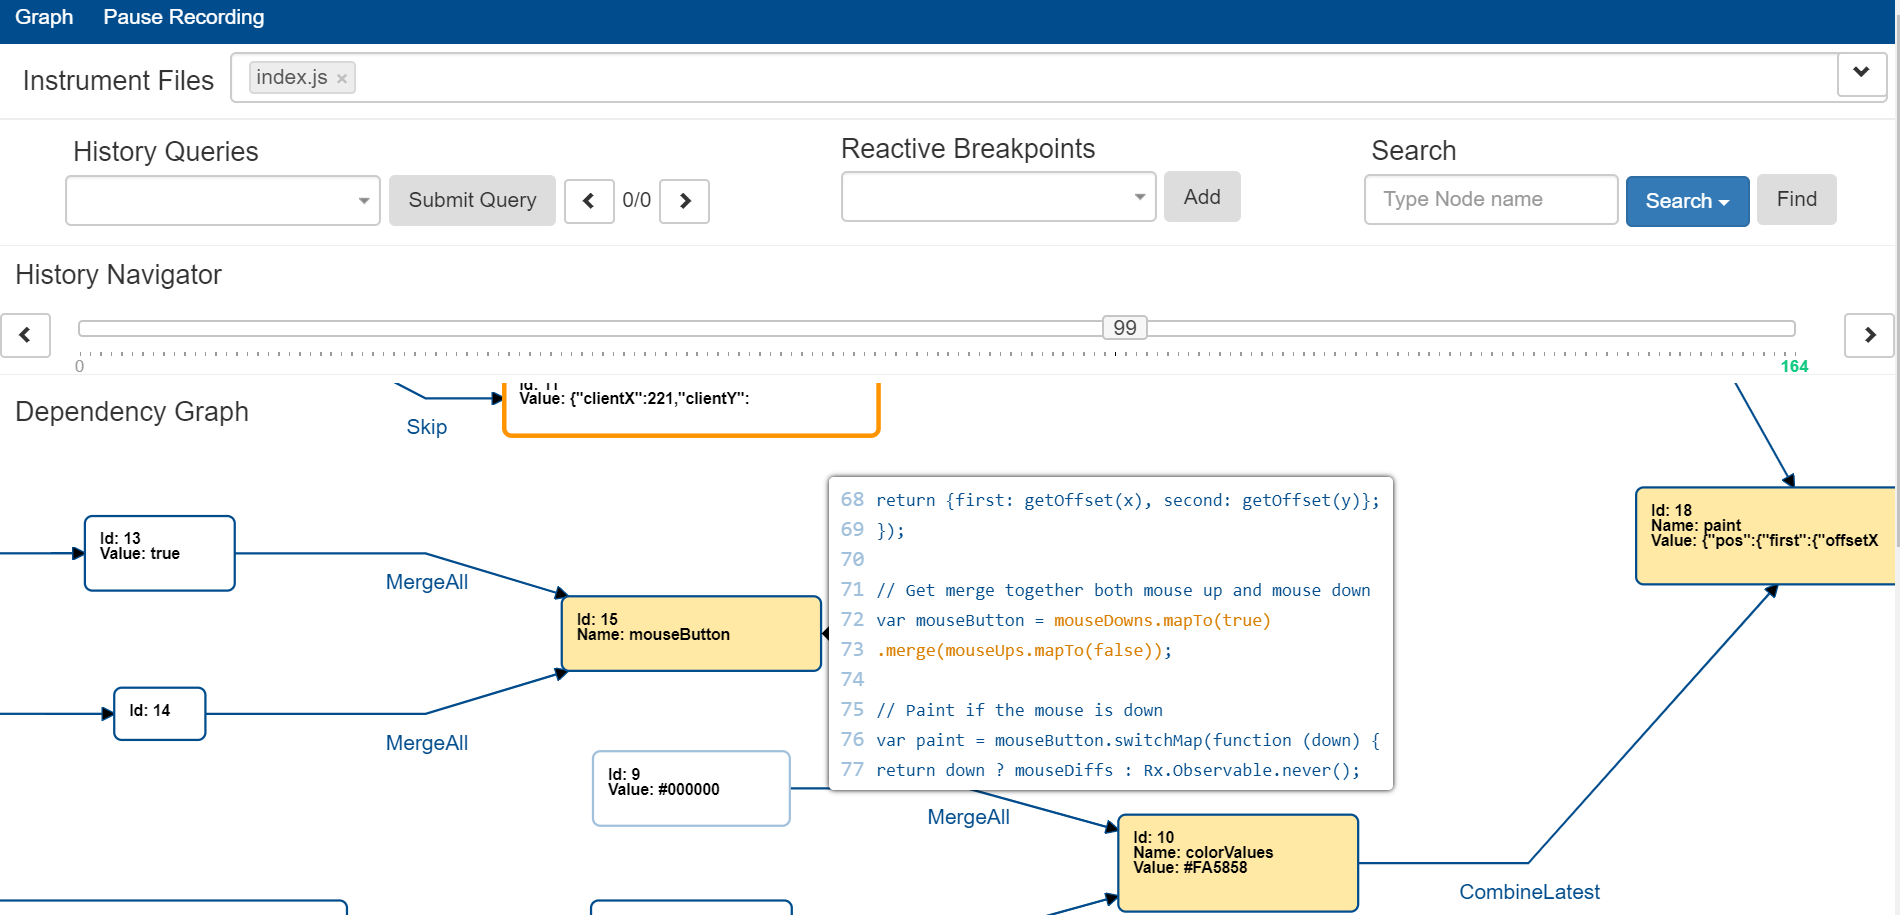
\includegraphics[scale=0.5,trim=0 0 0 0]{gfx/CRI-sampleView.png}
	\caption{A sample of CRI3 UI with opened Source Code Tooltip.}
	\label{fig:CRI}
\end{figure}

We made several additions to the UI of the CRI in order to show the Source Code Tooltips in the way described above. The class TooltipManager (located in tooltips.js) handles the creation and displaying of tooltips for all nodes in the dependency graph. It adds the UI events used to switch out the tooltips and requests the code needed to construct the Source Code Tooltips from the instrumentation script if the tooltip was not opened before in this step for that specific node. The used tooltip library tipsyJS \cite{Tipsy} which was used in previous versions of the CRI is no longer actively developed. We still decided to continue using it, because it provides a simple way to swap out tooltips as it accepts functions for any of the options passed as parameters to the library. However, we had to modify the library to include a fix for a rendering issue that was already submitted as a pull request to the GitHub repository of that library but not accepted due to not being actively developed anymore. In addition, to enable the capturing of keyboard events for the dependency graph it is necessary to explicitly make the containing HTML element focusable. This is done by adding a \emph{tabindex} attribute. Since the container also needs to have the keyboard focus in order to receive the keyboard events, the container is automatically focused when the user moves the mouse pointer over the dependency graph. The mouse events used to open or close a Source Code Tooltip of a node are registered when the user hovers over the node and removed when the mouse leaves the area of the node. We also chose to give the user a visual clue if a node has a Source Code Tooltip. This prevents users having to probe each node if a Source Code Tooltip is available. The border of nodes that cannot be linked to a source code position is, therefore, displayed faded. We chose this specific visual representation, because having no Source Code Tooltip for a node means the node does not provide any context information and the normal tooltip will most likely also not provide any valuable information. One could argue that the Location information could now be omitted from the normal tooltips as well, but it is currently the only way for the user to see from which JS file the node originated since Source Code Tooltips currently do not show the filename. However, this may be changed in the future. An example of the CRI UI with an opened Source Code Tooltip can be seen in figure \ref{fig:CRI}.
	
\section{Rapidly updated Observables}
\label{sec:RapidlyUpdatedObservables}
In this section, we discuss the difficulties when handling applications with rapidly updated observables and our approach to increasing the CRI's ability to cope with them. If the value of one or more observable is changed rapidly, each change will result in a new step in the dependency graph's history. Observables that are, for example, created from timers, mouse movement or a network connection submitting messages, change their value very often in a short period of time. The previous version of the CRI is not able to handle rapidly updated observables well. For a detailed performance comparison, see chapter \ref{ch:Evaluation}. However, there were two features added to the CRI that enable the user to still use the CRI with rapidly updated observables to some extent. One feature is the option to pause the recording and resume it at a later time. This feature is useful for applications which run some time before the limits of the CRI are exceeded and allow the user to click the \emph{Pause Recording} button before that happens. The user is then able to examine the recording up to this point without any issues related to performance. This is due to the fact that user interaction is slow enough for the CRI to handle, while steps may be generated by the thousands in the same period of time if the recording is not paused. The other feature that was added is the ability to exclude certain nodes from the recording process, although this is cumbersome to do. The user has to detect and remember the Ids of nodes which are being updated rapidly and then add these Ids to a list located on the options page. This ad-hoc solution can still be useful in certain cases, but in others, the full exclusion of a node will cause errors in the recording process or show a disrupted dependency graph. In the following, we explain the increased demand for resources, the steps implemented to increase performance in this thesis and the limitations of the UI in handling these type of observables in general.

\subsection{Difficulties and previous approach}
Not only does the generation of hundreds of steps decrease the expressiveness of each individual step, with some exceptions, but it is also very demanding on computational resources. Messages between content scripts, background scripts, and the extensions panel have to be transmitted in addition to saving the dependency graph's history. This also increases the number of rendering operations of the graph itself which requires a lot of size and position computations. If the computational effort exceeds the capabilities of Chrome and the underlying system, the CRI and sometimes even Chrome itself will stop working. There is a threshold regarding the minimum time span between individual updates that if undercut leads to the CRI crashing at some point of the execution. The reason for this is the accumulation of requests if more requests are submitted, for example to the Chrome message or storage API, than requests are processed. Over time the resource demand on scheduling requests and managing the JavaScript runtime's event queue increases beyond the available computation power. In this case, the UI becomes unresponsive and Chrome will eventually terminate the extension. In the remainder of this thesis, we will refer to this type of performance issue as \emph{request buildup}.
The steps that are often still significant to a user belong to the start of the history. They usually contain some form of setup phase, were observables and their dependencies are created, but there are no values submitted to them yet. An example of this is visible in many of the test applications, as value updates will not occur until the user starts using some form of input element. These steps can still be examined and provide valuable information about the created observables that is not value-update related. This setup phase, however, is not present in every Web application. If the application does not have a setup phase, the history becomes hard to examine. Even if there is a setup phase some parts may be implemented with something like the \emph{Lazy Loading} Pattern \cite{Lazy} in which the creation of observables will just happen on demand. There may also be no setup at all. It is possible to create observables dynamically - i.e. the type of dependencies used are a result of some form of computation or configuration - which will not necessarily happen at the start of an application. Another case in which the history becomes hard to examine for a specific task is if the application has multiple busy phases. Such an application may wait for some message from an external component that results in many computations and updated observables. Since the history does not provide an actual timeline and will show steps in a linear sequence these busy phases become very hard to identify and distinguish. 
Another difficulty that stems from the \emph{Pause/Resume Recording} features, is that pausing the recording leads to a broken history. There is no visual feedback in the history navigation that signals the user a pause has happened at some point in the history. If the recording is paused and later resumed, the steps before and after this gap are not sequential anymore, even though the history indicates the contrary. After the recording was paused, the dependency graph will actually show a false image of the variables as their value may differ from the actual variables in the application. This difference only persists until every node is updated once again, but if an observable or dependency is created during the pause, it will not be visible at all. The later is somewhat intentional for excessively, dynamically created observables discussed in section \ref{sec:DynamicallyCreated}. But this still leaves the user to remember at which step they paused the recording or they will get confused if they examine the dependency graph while stepping over the gap.
	
\subsection{Reworking the dependency graph History}
To reduce the computational resources required to record the dependency graph's history and implement a more sophisticated storing mechanism, we reworked the previous implementation. The history records every change to the dependency graphs as a new step. While previous versions of the CRI stored the whole graph for each step inside an array for simplicity. This means the required memory will increase proportionally with the number of steps. However, the overall memory consumption will not exceed the limits of the environment except in extreme cases, because modern computer systems normally have more than 1GB of RAM available. We decided to use Delta Encoding to reduce the required computations to store succeeding steps. The term Delta Encoding simply describes that instead of storing the full \emph{state} of some entity, for example an object, only the difference to the previous state is stored. This difference is called the Delta and in the case of the CRI the \emph{state} is the dependency graph in a specific step of the history. The Delta represents the change to the dependency graph from one step to the next. This approach is very useful to reduce the size of data that needs to be stored for any stream of data where the Delta between elements in the stream is marginally smaller than an element itself. It is used with great success in video encoding, because the difference between succeeding frames is usually very small, but depending on the resolution of the video, each frame can contain a large amount of information.
As the first step towards implementing Delta Encoding, we modularized the history and introduced \emph{Paging} to it. Although the term \emph{Paging} may be misleading as it usually refers to memory management of the operating system \cite{PagingWiki}, we use it to describe a software engineering pattern as it best describes our approach. This pattern is commonly used to handle large streams of data. What we refer to as \emph{Paging} is the implementation of a (software) cache to the history that loads a subset of succeeding steps. The history will only store a fixed size of steps at once. As soon as the size of this cache is exceeded, a part of the loaded steps is written to the local disk using the Chrome storage API and removed from the cache. The cache is in fact better referred to as a Page, because its content always consists of sequential steps while a usual (software) cache used in programming may contain elements in a random order. If a step is requested that is not currently loaded in the Page, the requested step is loaded along its surrounding steps from the Chrome storage API. The requested step is loaded as the middle of the Page, if possible, to prevent the need to immediately load another step from the local storage, if the user clicks next or previous. This approach keeps the memory consumption of CRI fairly constant and independent of the number of steps in the history, as the maximum number of loaded steps is the size of the Page. We built the Delta Encoding on top of the Paging, to keep the benefits of both approaches.
As mentioned earlier Delta Encoding reduces the data stored to the changes between succeeding steps. These changes are also the relevant information a user of the CRI examines when working with it. Therefore, storing these changes and their types actually provides more useful data and makes the changes easier to query. With the previous approach, the changes between steps needed to be calculated or logged in addition to the history as it was for the history query feature. For the same reason we implemented Delta Encoding ourselves instead of using a JSON Patch \cite{JSONPatch} based library like the one developed by \emph{Joachim Wester et al.} \cite{JSONPatchImplementation}. The library calculates Deltas itself which consumes additional resources. Delta Encoding also enabled an easy and more robust way to detect the current changed node, and later edge, instead of storing the highlighting in the graph itself. The current change in a step is simply the node or edge affected by the last Delta. With the simplest form of Delta Encoding, a specific step of the history would be created by loading the very first step and then applying all changes stored as Deltas in sequential order on the dependency graph stored in that first step. To reduce the computational cost needed to reconstruct a dependency graph for a certain step, we implement an algorithm similar to the one explained at \cite{VideoEncoding} without B-frames. We call the I-frames \emph{Base Stages}, which store a full graph, and P-frames \emph{Delta Stages}, which only encode the Delta to the previous step. The size of the Delta Window can be configured in code and is currently set to 100, meaning each \emph{Base Stage} will be followed by 100 \emph{Delta Stages} before a new \emph{Base Stage} is created. The implementation is located in \emph{history.js}. Paging is used to load a subset of continuous \emph{BaseStages} all at once and store the rest with the Chrome storage API. This is important in order to cope with the user stepping forward and backwards repeatedly over the threshold between two \emph{BaseStages}, which would be very resource demanding if only one \emph{Base Stage} would be loaded at once. Increasing the Page size also reduces the number of storage and load commands submitted to the local Chrome storage using the API. The Deltas are used on the graph level and, therefore, always contain the full node or edge that was changed or added, in contrast to value-based Deltas. As not all changes to the graph are easily reversible their Deltas always belong to the proceeding \emph{Base Stage} and not to the succeeding \emph{Base Stage}. This is also the reason we did not implement B-frames as used in the original algorithm. To keep the \emph{Delta Stages} that succeed a \emph{Base Stage} linked to it, we store them as part of the \emph{Base Stage} themselves. If a new \emph{Delta Stage} is added or requested that is in the forward direction in regard to the sequential order of the steps, without crossing over any \emph{Base Stage} boundaries, all changes are directly applied to the current loaded dependency graph. If, however, the direction is backwards, the new graph is constructed by emptying the graph, loading the \emph{Base Stage} and then applying all Deltas up to the requested stage. The same logic is used if a random step is requested that is not part of the current Base Stage. This means that loading steps in the forward direction, is always faster than accessing steps at random or backwards. As noted above the forward direction is crucial for the recording process and has a great impact on the performance of the CRI when handling applications with rapidly updated observables. The used algorithm and implementation keep this use case fast and simple. On the other hand, stepping back and the random access of steps requires additional computation in comparison to the previous implementation of the history. However, they are only ever triggered by the user themselves which greatly lowers their performance requirements.
The \emph{GraphManager} class handles drawing of the displayed dependency graph in the UI and request the loading of a different step from the history when necessary. It also implements the highlighting of the current node or edge. The \emph{History} class handles the actual data, caching and requesting loading of steps from the storage when necessary. It also manages when to switch to the next \emph{Base Stage} instead of adding another \emph{Delta Stage}. The shared, singleton object \emph{stageStorage} provides an Object-Oriented interface, that loads and stores \emph{Base Stages} with their \emph{Delta Stages}, to the key-value based Chrome storage API. \emph{stageStorage} also schedules request internally to ensure that they are handled sequentially and in the correct order. Guaranteeing that stages finish saving before the loading operation is executed. For this reason, the loading operation is asynchronous and uses a callback that is invoked when the loading is done. To achieve the synchronicity of these operations, \emph{stageStorage} uses a queue internally. If an operation finishes storing or loading it will invoke the next operation in the queue.	

\subsection{Additional performance improvements}
\label{sec:additonPerformance}
To further increase the performance of recording new steps in order to enable using the CRI with faster updating observables, we inspected the resource consumption with memory analysis as well as CPU profiling tools. A comparison of these inspections for the CRI3 and the previous version of the CRI is shown in chapter \ref{ch:Evaluation}. We discovered, that for applications with rapidly updated observables, a huge amount of CPU resources were spent on computations responsible for rendering positions and sizes of the Scalable Vector Graphics (SVG) HTML element used to display the dependency graph. A rendering operation was triggered for each newly created step in the history. Throttling these rendering operations and UI updates greatly increased the performance of the CRI. Since humans are not able to detect and comprehend changes to the UI happening faster than a certain threshold, decreasing the rendering operations to this threshold will not even be noticed by a user. In fact, we increasing the interval until the next rendering operation is triggered even further. The goal was to use an interval compromising between delay that a user notices and computational resources used to render the graph that often. According to an article by Thomas Burger \cite{Perception} the average human reaction time to visual input is 250ms. Since the CRI does not rely on real-time interaction, although the recording process needs to fulfill real-time requirements to a certain degree, they claim that latencies up to 500ms are acceptable before the performance of the user is affected. If a requested result is displayed with a delay of 100ms, the user will experience it as an immediate result. Delays above that will be noticed, but will not annoy most users if they are lower than one second. In order to increase the performance of the CRI while not introducing any nuances for the user with applications the extension can easily handle without the throttling, we chose 230ms as a compromise. This is significantly lower than 500ms, but since some Web applications will change node values in intervals smaller than that, we decided to use 230ms as it provided the most fluent experience. In the future it is desirable to add a self regulating mechanism that increases or decreases the delay on demand of the inspected Web application. The lower boundary for the delay should still be 230ms as not to waste computational resources. However, for applications that require extensive resources like the test application \emph{RxJS mario}, there is no fixed upper boundary for the delay. Steps are created so fast that the user is not able to gather any useful information. The displayed dependency graph and especially the history will only be useful to examine when the recording is stopped. Therefore, up to that point in time, the UI is unimportant and the delay at which rendering is triggered should be increased accordingly. The upper bound in this scenario is not existing, although it has to be noted, that as explained by Thomas Burger in the article \cite{Perception}, the users performance to perform a task will suffer from the delay until the recording is paused.
There is also the option to exclude some nodes from the recording introduced in the CRI1. This is effective if the application only has a few rapidly updated observables. For most applications with these type of observables, however, usually many observables have dependencies to one or more of the rapidly updated observables without filtering the submitted values. This leads to chains of rapidly updated observables that all need to be ignored to drastically reduce the number of generated steps. At this time, the CRI does not provide any tools to support the user in ignoring any observables. Some of the options in this regard are discussed in chapter \ref{ch:Future} and may be the target of further development.

\section{Excessively created Observables}
\label{sec:DynamicallyCreated}
This section discusses the origins of excessively created observables as well as some of the possible solutions to handle them, however, the implementation of these solutions is outside the scope of this thesis.
In addition to observables that are rapidly updated, another type of observable is difficult to handle for the CRI and similar tools. If new observables are created excessively, for example as part of a loop, the dependency graph is flooded with new nodes belonging to those observables. An example where this issue would occur is a Web application that uses networking to connect to a list of clients. The network clients each create an observable and each message submitted to one of them is gathered in a single observable that depends on them. If many clients connect or reconnect to the Web application, the dependency graph becomes very large and hard to examine. We refer to excessively created observables as a special type of a observable for simplicity, although technically the term describes a group of observables that are created from the same source code. Since these type of observable usually stem from the same line of source code, the nodes will all share their detailed information like the source position information or name, except for their value. In addition to many long-lasting observables, the same issue occurs if observables are created temporarily, for example, as part of a function that performs some type of calculation. Since the CRI does not detect if observables are no longer used, the dependency graph shows nodes even after they were deleted by the garbage collector. Another issue for these type of observables is that if their nodes have a \emph{name}, the current implementation of the CRI's history query and search feature cannot distinguish them properly because the node identification for some of the queries are based solely on the \emph{name} and does not consider the scope the variable belongs to.
There is no simple way to exclude or handle this type of observables, as they have numerous sources and behaviors that need different solutions. All possible solutions have in common that they increase the complexity of the recording process.

\subsection{Increased recording complexity}
To exclude nodes from the recording of rapidly updated observables the user is able to specify Ids of the nodes to ignore. However, this approach does not provide a solution for excessively created observables, since instead of updating existing nodes, new nodes are created. For \emph{named} nodes the exclusion is possible using the name, but this does not work for any other nodes. For this reason, the CRI has to provide rules that specify certain characteristics by which newly created nodes are filtered. In contrast to ignoring the value updates and still creating the nodes, this type of observables has to be excluded from the recording process completely. Yet, some visual representation of these nodes is required in the dependency graph. Detection of nodes that belong to excessively created observables needs to handle many subcategories of these observables. One possible solution is to replace the group of nodes with a single pseudo node that merges all nodes of the group. This is not suitable for all categories of excessively created observables and is only applicable if all outgoing edges have the same target and ingoing edges have the same source. For cases in which these differ, the edges may be displayed with a sophisticated visual graph optimization approach like edge bundling \cite{EdgeBundling}. In this approach, the values of the merged nodes are displayed on the pseudo node. These values cannot be omitted in general even though they differ for every observable in the group and one group may consist of hundreds of nodes, depending on the inspected Web application. To display these values a scalable UI element is needed that allows the user to inspect any of the values independent of the group size. The detection of nodes to merge into a group is fairly robust when using the source position, although there may be some other cases in which nodes should be merged. As we mentioned earlier there are several possible options to handle these type of observables, but all have in common that the recording process increases in complexity. If the user should be able to reverse the merging of nodes on demand or a rule-based exclusion is chosen as the approach to handle this issue, the recording becomes customizable. To enable the user to keep the customization over more than one session, it has to be persisted. Since the customization is also highly specific to a single inspected Web application, some form of session or project management. In contrast to the current implementation of excluding nodes via the options page, the loading and storing of this persistent customization should be integrated into the menu of the main UI, because it directly corresponds to the currently displayed dependency graph.
	
\section{The Chrome Reactive Inspector - A growing project}
At the beginning only one developer, Waqas Abbas was working on the project who was later joined by Pradeep Baradur. They worked independently but parallel for some time and both extended the CRI as discussed in section \ref{sec:PreviousCRI}. Their work on the CRI was strictly focused on implementing the basic extension itself and then extending it with many features. However, as the project grew and their work later was merged as the first task of this thesis, the focus moved the CRI to be a full-fledged project that introduces new maintainability and extensibility requirements. In this section, we describe our approach to increasing development velocity and those requirements by reorganizing the file structure and increasing modularity.

\subsection{Increasing velocity}
In the CRI1 the JS files of the extension were mostly organized into directories with files that implement similar or related functionality. For example, all files containing the code corresponding to the recording of nodes from the reactive libraries were located in the \emph{event-sniffer} directory. As we started working on the project, we discovered that this organization is not suitable at the top level, because it most likely confuses any developer working on the project. The reason for this is the different contexts in which JS files are executed in a Chrome extension. The \emph{window} object representing the global scope of a JS file can be different to the one used in other files. The \emph{window} object in a content script is shared among all content scripts and provides access to the Document Object Model (DOM) of the inspected Web application. However, the \emph{window} object in JS files that run in the context of the DevTools panel of the CRI is specific to that context and provides access to the DOM of the CRI's panel. Background scripts also have their own shared context. In addition, scripts running in these different contexts have access to other subsets of the Chrome API. If the JS files of the extension are organized as in the previous version of the CRI, JS files located in the same directory may run in different contexts. To remove this confusion, we separated the JS files at the top level by their context. Background scripts are located in the \emph{background} directory while content scripts are located in the \emph{content-scripts} directory. The scripts that run in the context of the DevTools panel are located in the \emph{devtools} directory. All external libraries are located in the \emph{libraries} directory because some libraries are used in multiple contexts. At any level below the top level separation by context, the scripts are still organized into directories with files sharing similar or related functionality. This reduces the risk for a developer to lose track of the \emph{window} object and access to the Chrome API available for a script.
A large part of documentation for the previous versions of the CRI was included in the theses of Waqas Abbas and Pradeep Baradur, however, the number of comments directly providing documentation within the source code were sparse. A developer starting to work on the project had to check the external documentation to comprehend the source code, increasing the time required to do so. Therefore, to further increase development velocity we also added additional source code documentation to reduce the time needed to comprehend the existing code. We measured the number of single- and multi-line comments for both the Chrome Reactive Inspector version 2 (CRI2) created by Pradeep Baradur as part of his thesis and the current version of the Chrome Reactive Inspector, version 3 (CRI3), to verify that the number increased. The source code of the CRI2 contains 231 single- and 32 multi-line comments while the source of the CRI3 contains 271 single- and 52 multi-line comments. These numbers include TODO comments, found mostly in the CRI3, and commented code, found mostly in the CRI2. Only JS files developed in the CRI were included in the measurements. 
As the project grew and more and more features were added, some JS files grew above 500 lines of code, for example, \emph{panel.js}. In mind of software engineering aspects like separation of concerns and modularity, long files with multiple independent tasks are not desirable. In addition, the nature of JS as a script language without class definitions (before ECMA6) tempts developers to neglect encapsulation and use many global variables and functions. To increase modularity and encapsulation, which helps to track and correct errors or extend existing code by enclosing the influence of a change or limiting the code that has to be inspected for a specific error, we used the JS closure pattern. A closure prevents variables to be accessed from the outside and makes them effectively private. This works because variables are bound to a function context in JS. In the example seen in listing \ref{lst:closure}, a self-executing function is used to implement the closure pattern that returns a function. It is also possible to use closures to create pseudo-classes in JS that can be instantiated with the \emph{new} keyword. In that case, the self-executing function returns a constructor function that in turn return an object. In addition to both these construct, we used closures to implement singleton objects. An example for this is the \emph{stageStorage.js} file. Using closures prevents the pollution of the global window object (for a specific context) while also documenting that these functions belong together. In addition, they limit the interface to other components of the application to a set of explicitly public variables and functions.
		\begin{lstlisting}[language=JavaScript, caption={Example of RxJS code.},label={lst:closure}]
			var add = (function () {
			var counter = 0;
			return function () {return counter += 1;}
			})();
		\end{lstlisting}
In total, we added nine new classes. The only JS scripts that are still not using a closure to encapsulate their internal logic are the files \emph{background-communication}, \emph{options}, and \emph{panel}. The first two are the only scripts inside their respective context. The \emph{panel} script ties all features together and previously used and provided many globally accessed variables. This increased the development effort to separate individual components and dependencies beyond the scope of this thesis as this was not its main focus. Although several efforts have been made to move some components to their own JS files and to reduce the number of global variables. In the future, the code responsible for the search and history query feature is to be extracted too. Ultimately the \emph{panel} should only be responsible to instantiate other classes and delegate events and tasks to them. To further increase modularity and provide developers with a robust and tested pattern for separation of concerns in application with a UI, a common pattern like Model View Controller (MVC) or Model View ViewModel (MVVM) should be used for the CRI DevTools panel.
Code metrics are usually used to verify that modularity and separation of concerns are adhered, while still avoiding high coupling of these modules. However, most code metrics like coupling and cohesion \cite{Coupling} cannot be calculated for a dynamically typed language like JavaScript. Instead of these metrics that provide sound results for Object-Oriented programming, we used more ad-hoc and less robust metrics. In detail, we used the total number of lines, the number of files and the average number of lines per file to provide insight on the extent to which we increased modularity. See the Appendix \ref{ch:Appendix} for the exact results.
	
\subsection{Build process}
The CRI provides a packed Chrome extension file that is deployed as the stable version. This packed extension contains by default all files in the chosen subdirectory, including files that are only relevant for developers of the CRI like the \emph{.gitignore} file in addition to IDE project files that may even expose sensual information about developers or their development systems. The suggested approach is to implement a custom build process that creates a new directory that only contains files need to run the extension \cite{BuildScript}. We implemented the build process in JS using \emph{NodeJS} \cite{NodeJS} in the \emph{build\_process} project. The reason to use a JS build script in place of any other sophisticated build language is to provide the developers with a familiar language and tools. In the future, this build process may also be used to reduce the size of the CRI's JS files by minifying them. 